\chapter{Processing of electron backscatter patterns}
\label{chap1}

Electron microscopes are used in many scientific fields to study microstructure of materials. They rely on electrons instead of photons, which allows them to achieve greater magnification than light microscopes. The microscope emits a beam of electrons, which interact with the specimen, either transmitting through it or reflecting back. The electrons therefore carry an information about the specimen. We capture them on a phosphor screen which emits light and then we take a picture of the screen by a camera, so the result of one electron microscope measurement is an image.

One measurement of electron microscope gets information about only one microscopic point in the specimen. However sometimes we need to map a larger area of the material. For this purpose, scientists use a \emph{scanning electron microscope}. It is a device that repeatedly emits an electron beam towards the specimen, scanning the surface in a raster pattern. So it does the measurement in one place, then moves a bit (e.g. $\SI{1}{\nano\meter}$ aside) and repeats. Since we are measuring the micro world, it takes thousands of iterations to scan a reasonably large area of the specimen. For example, test data that we used contained over 15000 images taken in a $120 \times 120$ raster covering an area of the specimen surface approximately $\SI{70}{\nano\meter} \times \SI{70}{\nano\meter}$ big.

We process data obtained using the \emph{electron backscatter diffraction} which is a scientific method that utilizes the scanning electron microscope to study crystalline materials (i.e., materials with a highly ordered microscopic structure). The principle of the electron backscatter diffraction is sketched in \cref{ebsd-principle}. When a beam of electrons is emitted towards the specimen, some of the electrons backscatter, that is, they reflect back from the surface. They are then captured on a phosphor screen which is coupled with compact lens that directs the captured image towards a camera. The result of this procedure is a grayscale image of the \emph{electron backscatter pattern}. An example of such pattern is shown in \cref{roi-shifts:initial}. White color in the image can be interpreted as a place where many electrons were captured whereas black areas captured smaller amount of electrons.

\begin{figure}
	\centering
	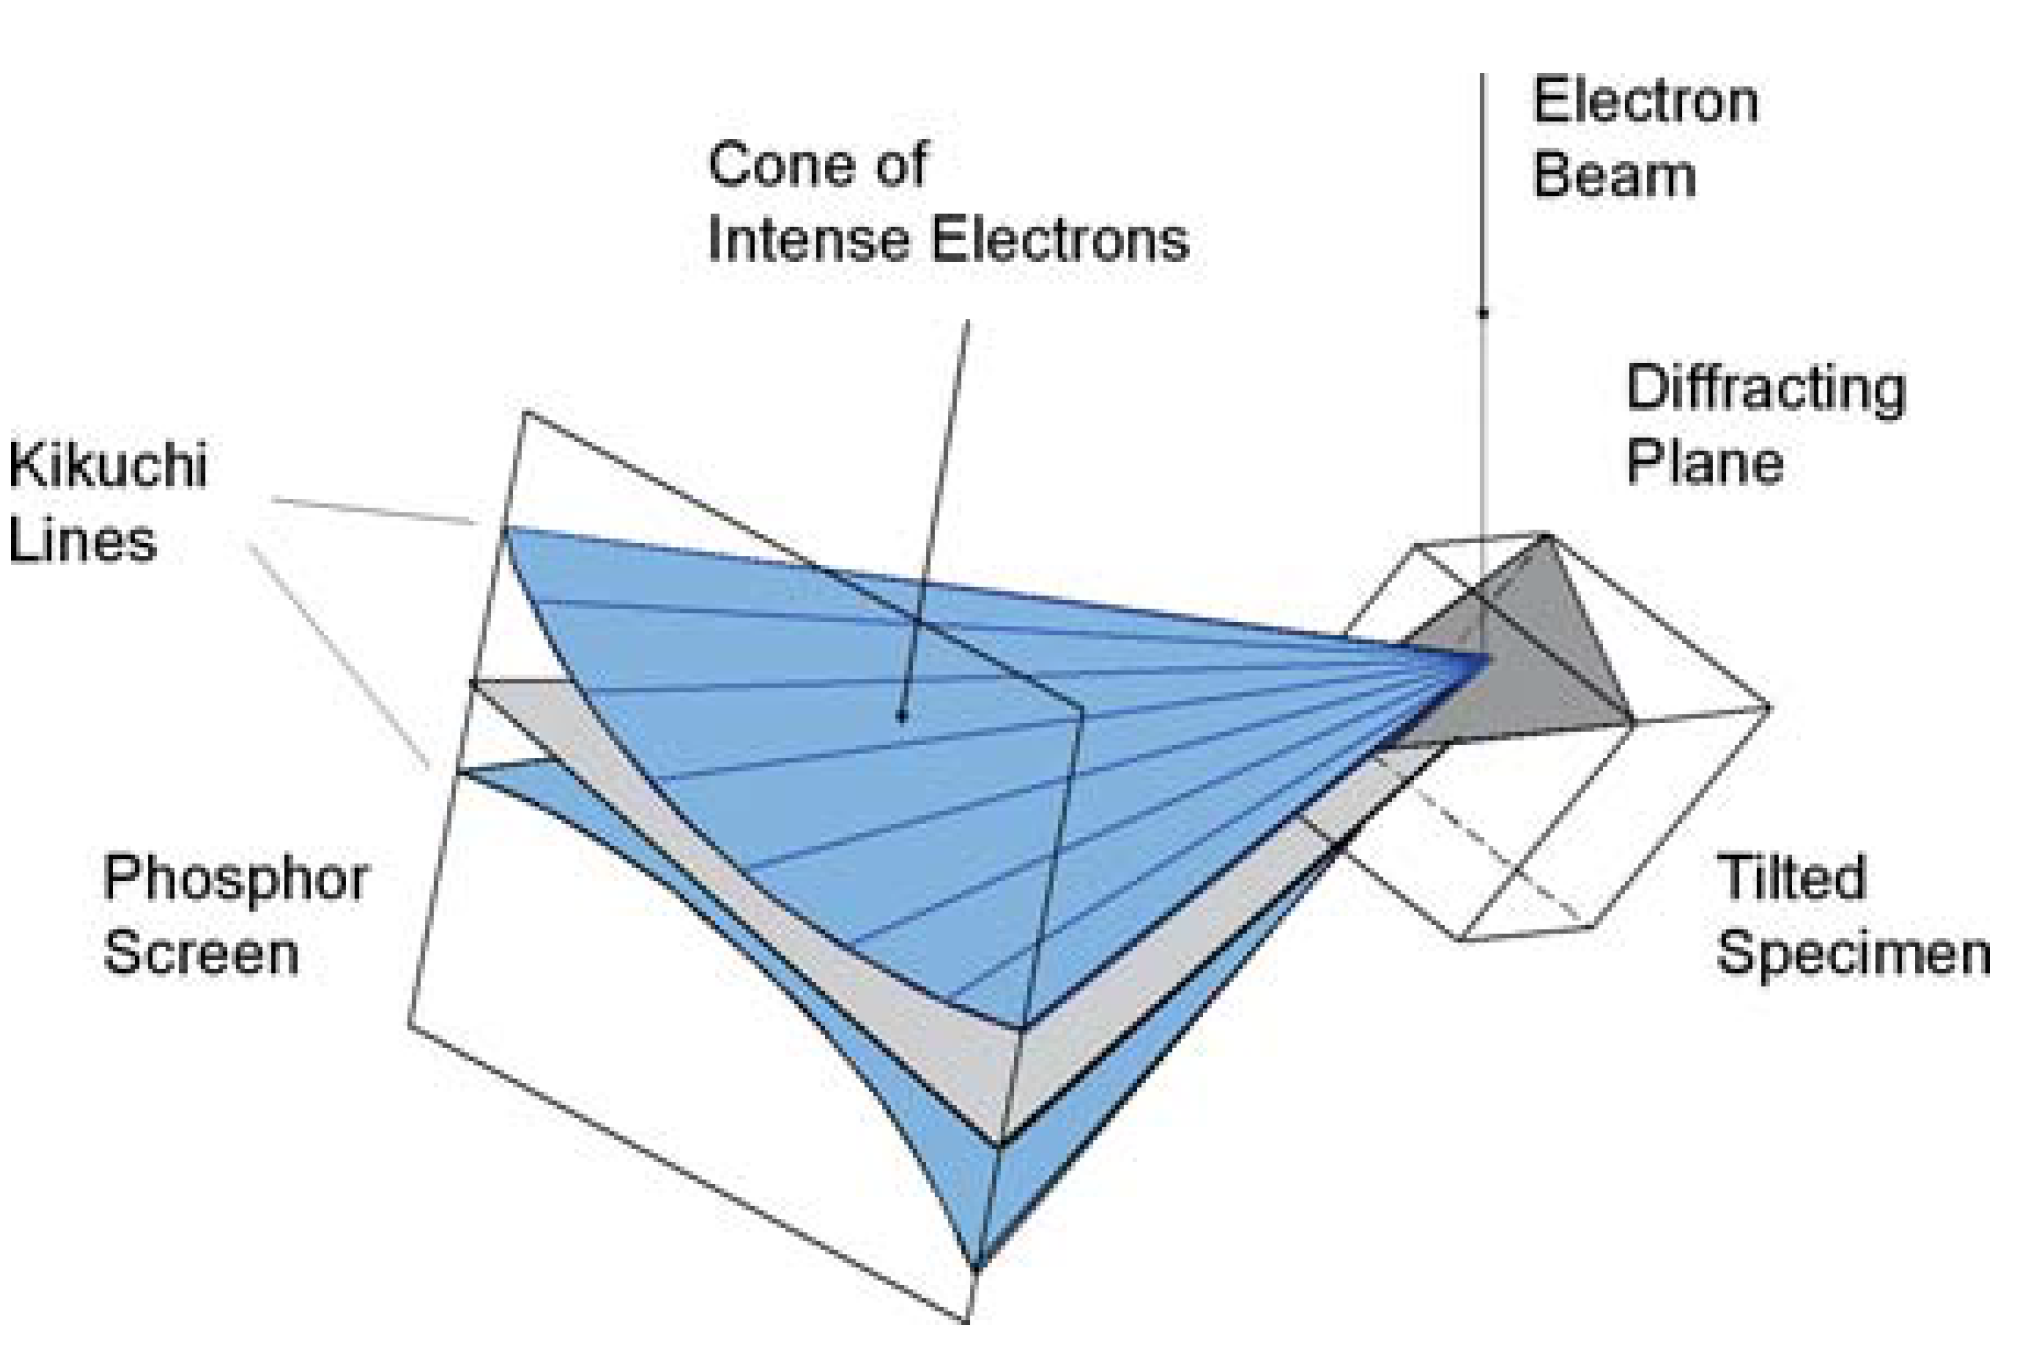
\includegraphics[width=0.6\textwidth]{img/ebsd_principle}
	\caption{The principle of electron backscatter diffraction. \cite{schwartz2009electron}.}
	\label{ebsd-principle}
\end{figure}

\begin{figure}
	
	\begin{subfigure}{.4\textwidth}
		\centering
		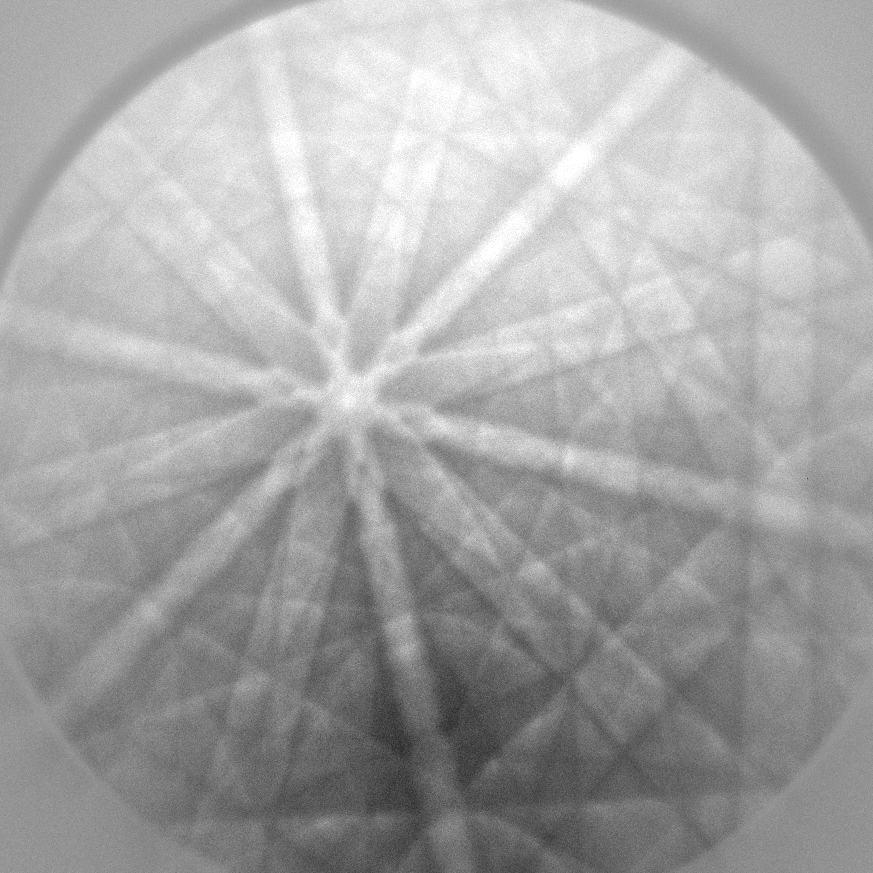
\includegraphics[width=.9\linewidth]{img/roi_shifts_initial}
		\caption{Initial, undeformed pattern}
		\label{roi-shifts:initial}
	\end{subfigure}%
	\begin{subfigure}{.4\textwidth}
		\centering
		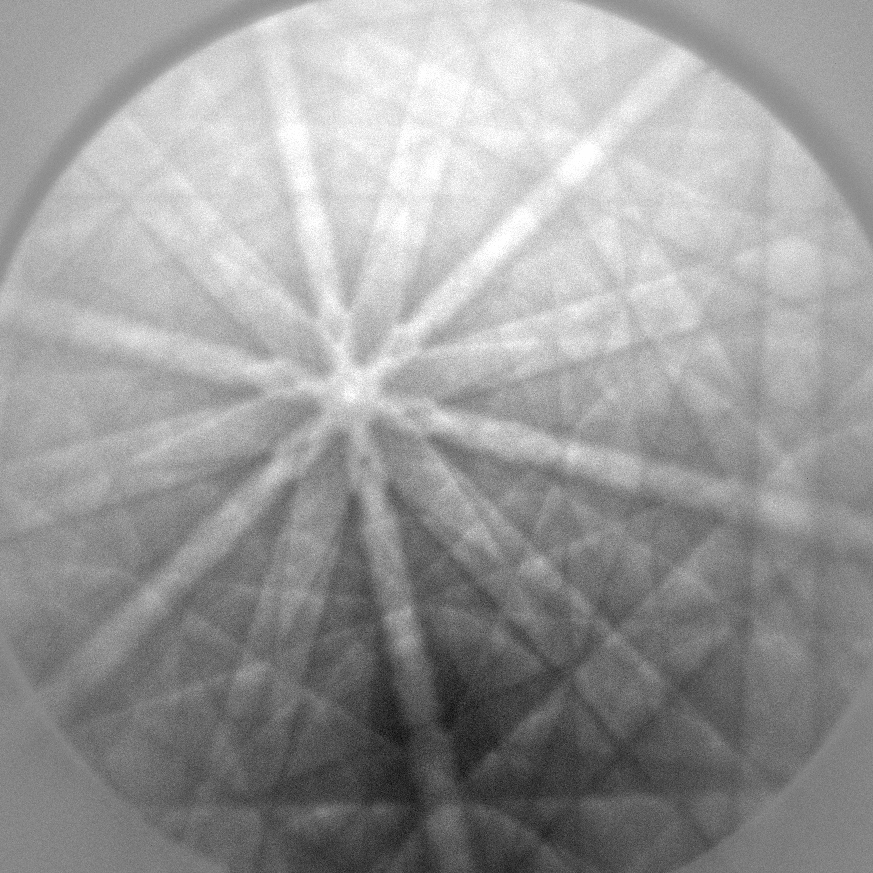
\includegraphics[width=.9\linewidth]{img/DEFORMED_x3600y6235}
		\caption{Deformed pattern}
		
	\end{subfigure}
	\centering
	\begin{subfigure}{.4\textwidth}
		\centering
		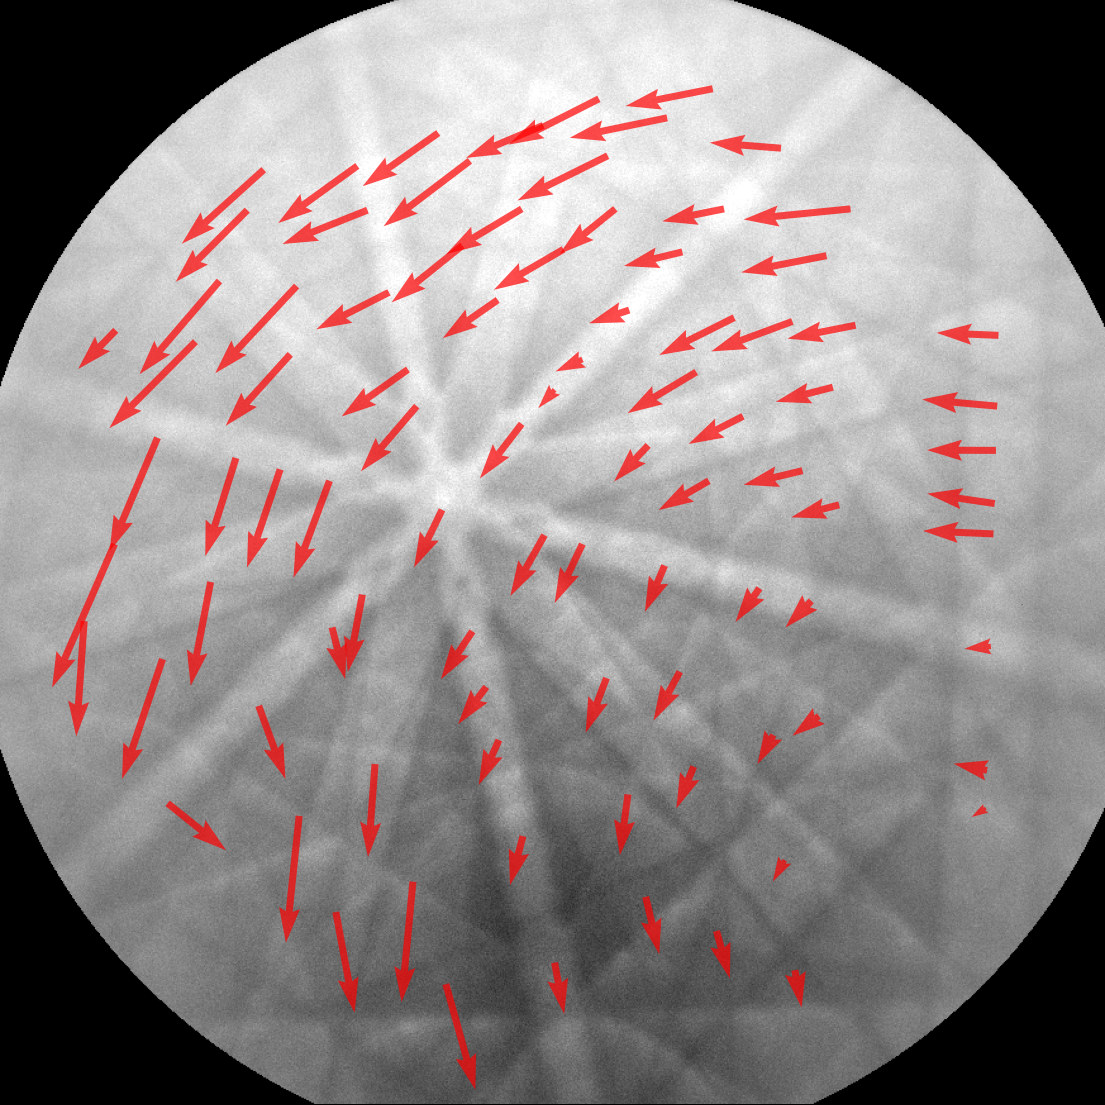
\includegraphics[width=.9\linewidth]{img/roi_shifts}
		\caption{Deformation visualization}
		\label{roi-shifts:result}
	\end{subfigure}
	
	\caption{Deformed pattern with arrows visualizing the deformation. The arrows are upscaled for the visualization, because the pattern is deformed only by several pixels (the biggest offset is less than 10 pixels long, while the whole picture has resolution $873 \times 873$).}
	\label{roi-shifts}
\end{figure}

The electrons do not reflect randomly, but based on the examined specimen, they backscatter in a specific way, forming \emph{Kukuchi lines} observable in the pattern. The geometry of Kukuchi lines can be interpreted as a projection of the specimen crystal structure on the flat phosphor screen.

When the crystal structure of material is changed (e.g. under stress), the deformation can be observed in the backscatter pattern as well. Therefore, the patterns of deformed specimen can be compared to undeformed ones to measure elastic strain and crystal lattice rotation.  \Cref{roi-shifts} shows a visualization of such comparison. Since different parts of the images may be deformed differently, a commonly used technique \cite{wilkinson2006high,wilkinson2010high,britton2012high} is to choose several (usually tens to hundreds) subregions of the patterns and determine the vector of shift between the corresponding regions from both patterns. The shifts estimate the real deformation of the crystalline structure.

The comparison is done by cross--correlating respective subregions of the deformed and reference patterns. The position of the maximum value in the correlation result determines the most probable shift with one pixel precision, which is not enough. To achieve subpixel accuracy, we estimate the peak of the cross--correlation by interpolating from a small neighborhood of the maximum.

Once the shifts are computed, they are further processed to obtain an estimation of the actual crystal deformation and other characteristics. However, we do not address that part of the analysis in this thesis, as it is not nearly as computationally expensive as the processing of the images. Moreover, the comparison is commonly used in analysis of the electron backscatter diffraction data, while the processing of the shifts may be different for various purposes.

To sum up, we have thousands images of deformed electron backscatter patterns. Each of them was captured by a scanning electron microscope at a specific location of a specimen. Moreover, we have one reference image of the electron backscatter pattern. We need to quantify the deformation of each deformed pattern, so we choose several subregions and cross--correlate each respective reference and deformed subregion. Maximal correlation gives us the most probable shifts of the subregions. So for each deformed pattern, the result of our algorithm is a list of shifts corresponding to subregions. The shifts are then further processed to obtain their physical interpretation, but that is not covered in this thesis.

%In this chapter we describe the algorithm used to analyze the deformation of the patterns. We define cross--correlation and least squares --- techniques that are used in the analysis. Finally, we describe the algorithm that we study in this thesis.

\section{Algorithm description}

In the rest of this chapter, we describe an algorithm used to process the electron backscatter patterns. The specifics of the algorithm correspond to a version that is used in Department of Physics of Material in Charles University in Prague.

The algorithm takes the following input and parameters:
\begin{itemize}
	\item reference image of electron backscatter pattern with size $W_p \times H_p$
	\item $N$ deformed images of electron backscatter pattern images, each with size $W_p \times H_p$
	\item $S$ positions of subregions that will be compared from each image
	\item size $W_s \times H_s$ of each subregion
	\item parameter $F$ that denotes the size of neighborhood used to interpolate the maximum with subpixel accuracy (see \cref{subpixel-peak})
\end{itemize}
The input images are all greyscale, which means each pixel is represented by one number. In our testing data, pixels were represented by 16 bit integers in range~$0 - 65535$.

The result of the algorithm is a list of $S$ shifts for each of the $N$ deformed patterns (see \cref{roi-shifts:result} for visualization of the shifts for one pattern).

Algorithm \ref{algo-whole-highlevel} shows a high--level pseudocode of the algorithm. It iterates through all deformed patterns and all subregion positions specified in the input. For each subregion, it computes the cross--correlation between the deformed subregion and subregion at the same position from the reference pattern. The result of cross--correlation is a matrix that expresses a measure of similarity for each possible shift between the subregions (see \cref{cross-corr-def}). In the next step, we further process the matrix to obtain the most probable shift with subpixel accuracy (see \cref{subpixel-peak}), which is the output of the algorithm.

\begin{algorithm}
	\caption{Processing of electron backscatter patterns}
	\label{algo-whole-highlevel}
	\KwIn{one reference electron backscatter pattern \newline
		$N$ deformed electron backscatter patterns \newline
		position of $S$ subregions from each pattern \newline
		size of a subregion \newline}
	\KwOut{deformation shifts for all $S$ subregions from all $N$ deformed patterns}
	\vspace{5px}
	
	refPat  $\leftarrow$ reference pattern\;
	\ForEach{\emph{defPat} in deformed patterns}{
		\ForEach{\emph{regPos} in subregion positions}{
			refReg, defReg $\leftarrow$ extract subregions from refPat and defPat\;
			
			crossResult $\leftarrow$ cross--correlate(refReg, defReg)\;
			
			maxX, maxY $\leftarrow$ subpixelPeak(crossResult)\;
			output [maxX, maxY]\;
		}
	}
\end{algorithm}

\section{Cross--correlation}
\label{cross-corr-def}
Cross--correlation provides a measure of similarity of two series for each possible shift between them. It is used in signal processing to find a shorter known feature in a signal or in image processing to locate a smaller shape in a bigger picture. In analysis of the backscatter patterns, it is used to find the most probable relative displacement between two images (subregions of images).

Cross--correlation of two discrete functions $f, g: \mathbb{Z} \rightarrow \mathbb{R}$ is a function $C:~\mathbb{Z} \rightarrow \mathbb{R}$ defined as follows:
\[
C[n] = (f \star g)[n] = \sum_{m=-\infty}^{\infty}f[m]g[m+n],
\]
where $\star$ denotes cross--correlation.

If $C = f \star g$ then $C[n]$ is a number that tells us how much are functions $f$ and $g$ similar, when $g$ is shifted by $n$ to the left. For each negative $n$, $g$ is shifted to the right. \Cref{correlation-example} shows two example functions and their cross--correlation.

\begin{figure}
	\centering
	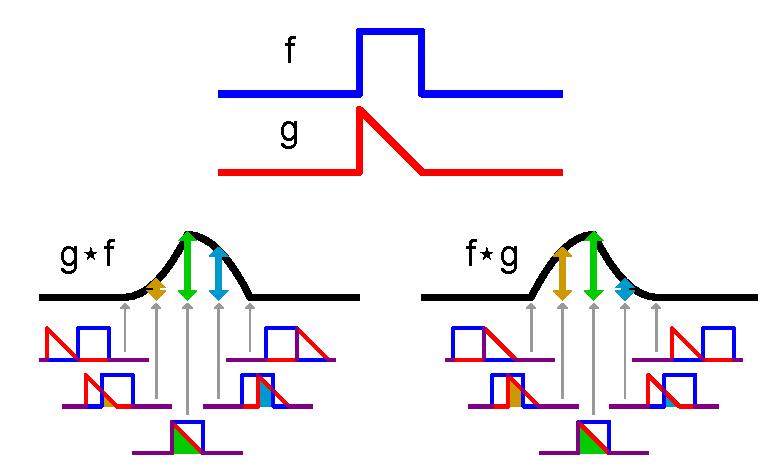
\includegraphics[width=0.7\linewidth]{img/correlation}
	\caption{The cross--correlation of two example functions\cite{correlation_example}.}
	\label{correlation-example}
\end{figure}

Definition of cross--correlation can be extended for two dimensions. For two--dimensional functions $f, g: \mathbb{Z}^2 \rightarrow \mathbb{R}$, their cross--correlation is a function $C: \mathbb{Z}^2 \rightarrow \mathbb{R}$ defined as:
\[
C[i,j] = (f \star g)[i,j] = \sum_{x=-\infty}^{\infty}\sum_{y=-\infty}^{\infty}f[x,y]g[x+i,y+j].
\]

Analogously to one--dimensional cross--correlation, $(f \star g)[i,j]$ is a number that is higher if $f$ is similar to $g$ shifted by $i$ horizontally and by $j$ vertically. \Cref{2d-correlation-example} demonstrates how cross--correlation can be used to search for a smaller pattern in a bigger picture. The brightest points (maxima) in \cref{2d-correlation-example-result} correspond to the best matches between the pattern and the image.

\begin{figure}[b!]
	\centering
		\begin{subfigure}{.49\textwidth}
		\centering
		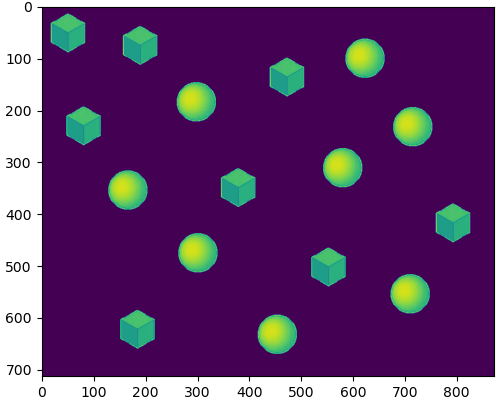
\includegraphics[width=\linewidth]{img/shapes}
		\caption{An image}
	\end{subfigure}
	\begin{subfigure}{.49\textwidth}
	\centering
	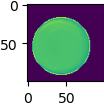
\includegraphics[width=0.4\linewidth]{img/shapes_pattern}
	\caption{Search pattern}
	%\label{fig:sub2}
	\end{subfigure}
	\begin{subfigure}{.5\textwidth}
		\centering
		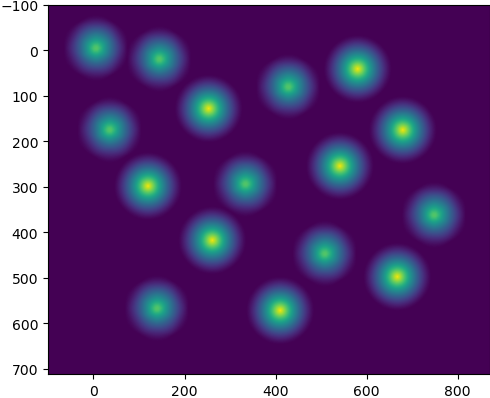
\includegraphics[width=\linewidth]{img/shapes_correlated}
		\caption{Cross--correlation of the (a) and (b) images}
		\label{2d-correlation-example-result}
	\end{subfigure}
	
	\caption{An example of cross--correlation used to find an object in an image. The maxima of the cross--correlation result correspond to the location of the search pattern (b) in the image (a).}
	\label{2d-correlation-example}
\end{figure}

Theoretically, the domain of cross--correlation is the whole $\mathbb{Z}^2$. However, when cross--correlating two images, i.e., real--valued matrices, $(f \star g)[i,j]$ does not make sense for all $[i,j] \in \mathbb{Z}^2$, because for some of them the images are shifted so much they do not overlap. For two images with sizes $w_1 \times h_1$ and $w_2 \times h_2$, the size of their relevant cross--correlation domain is $(w_1 + w_2 - 1) \times (h_1 + h_2 - 1)$. The result is a rectangle with the following corners: $[-w_1+1,-h_1+1]$, $[-w_1+1,h_2-1]$, $[w_2-1,h_2-1]$, $[w_2-1,-h_1+1]$. Those are the points of cross--correlation, where the result is computed from the images overlapping only by one pixel.

\subsection{Computing cross--correlation using discrete \\ Fourier transform}
\label{fft}

The cross--correlation can be computed using an algorithm based on its definition with asymptotic time complexity $\mathcal{O}(W_s^2H_s^2)$ for two images with resolution $W_s \times H_s$ --- for each of the resulting $(2W_s - 1)(2H_s - 1)$ pixels, we need to multiply at most $W_sH_s$ pixels. In the following section, we describe a way to compute two--dimensional cross--correlation in $\mathcal{O}(W_sH_s\log_2(W_sH_s))$ using \emph{discrete Fourier transform}. In the next section we show how it is used to compute \emph{circular cross--correlation}, which can be subsequently transformed into the (non--circular) cross--correlation we defined in the previous section.

%We first define \emph{circular cross--correlation}, because it can be used to compute cross--correlation. Then, we define \emph{discrete Fourier transform} and show how it is used to compute circular cross-correlation. Finally we show how to get the cross--correlation we need in the implementation. All is described for one--dimensional case only, since two--dimensional is analogous.

Let $N \in \mathbb{N}$, $\{x_n\} = x_0, x_1, \dots , x_{N-1}$ and $\{y_n\} = y_0, y_1, \dots , y_{N-1}$ be series of complex numbers. Then their circular cross--correlation is another series of $N$ numbers defined by the formula
\[
\{\mathbf{x} \star_N \mathbf{y}\}_n = \sum_{l=0}^{N-1}x^\star_ly_{(n+l)\bmod N},
\]
where $\cdot \star_N \cdot$ denotes the circular cross--correlation of two series.
%We can see that the definition is very similar to cross--correlation of two functions (see \cref{cross-corr-def}), except here we do.

Circular cross--correlation can be interpreted as a cross--correlation of two periodic functions. For any periodic function with period $N$, we only need $N$ consecutive values to represent, since the rest of the function repeats the same values. At the same time, given two periodic discrete functions $f, g : \mathbb{Z} \rightarrow \mathbb{C}$ with period $N$, their cross--correlation $f \star g$ is also periodic with the same period. So if we interpret the series in the definition of circular cross--correlation of as periodic functions, then the resulting series represents (non--circular) cross--correlation of the functions.

%The $\mod$ operation causes that whenever the $n+l$ is greater or equal than $N$, we ``circulate'' and take 

The circular cross--correlation can be quickly computed by using the discrete Fourier transform.

The \emph{discrete Fourier transform} is a function $\mathcal{F}: \mathbb{C}^N \times \mathbb{C}^N$ that transforms a series of $N \in \mathbb{N}$ complex numbers $\{x_n\} = x_0, x_1, \dots , x_{N-1}$ into another $N$ complex numbers $\{X_n\} = X_0, X_1, \dots , X_{N-1}$, which are defined as follows:
\[
X_k = \sum_{n=0}^{N-1} x_n \cdot e^{-\frac{i2\pi}{N}kn}.
\]
The Fourier transform is invertible, so if $\mathcal{F}(\mathbf{x}) = \mathbf{X}$, then $\mathcal{F}^{-1}(\mathbf{X}) = \mathbf{x}$.

Fourier transform has a broad range of practical applications --- it is used for example in digital signal processing, solving partial differential equations or big numbers multiplication. It can be used to quickly compute the circular cross--correlation using the following theorem \cite{proakis2004digital}.

Let $N \in \mathbb{N}$, $\{x_n\} = x_0, x_1, \dots , x_{N-1}$, $\{y_n\} = y_0, y_1, \dots , y_{N-1}$ be series of complex numbers and let $\{X_n\}$, $\{Y_n\}$ be their Fourier transforms. Then, we can compute \emph{circular cross--correlation} like so: 
\[
\mathcal{F}^{-1}\{\mathbf{X}^\star \cdot \mathbf{Y}\}_n = \sum_{l=0}^{N-1}x^\star_ly_{(n+l)\bmod N},
\]
where $\star$ denotes the \emph{complex conjugate} and $\cdot$ denotes element by element multiplication. Complex conjugate of a complex number $a + bi$, where $a, b \in \mathbb{R}$, is the complex number $a - bi$. Complex conjugate of series $\{a_n\}$ is series $\{b_n\}$, where every element $b_n$ is the complex conjugate of the original element $a_n$.

In other words, in order to compute the circular cross--correlation of two series $\{x_n\}$ and $\{y_n\}$, we first compute their Fourier transforms $\{X_n\}$ and $\{Y_n\}$, then multiply corresponding elements of the complex conjugate of $\{X_n\}$ and $\{Y_n\}$. Finally, we do an inverse Fourier transform. We do all of this, because we are able to compute both the discrete Fourier transform and its inverse in time $\mathcal{O}(N \log N)$, which gives us the overall asymptotic time $\mathcal{O}(N \log N)$ compared to $\mathcal{O}(N^2)$ when computing the circular cross--correlation from definition.

%To compute non--circular cross--correlation using this method, we use a trick with zero padding. Let $N \in \mathbb{N}$, $f$ and $g$ be two discrete functions, that are non--zero only in the first 

\begin{figure}
	\centering
	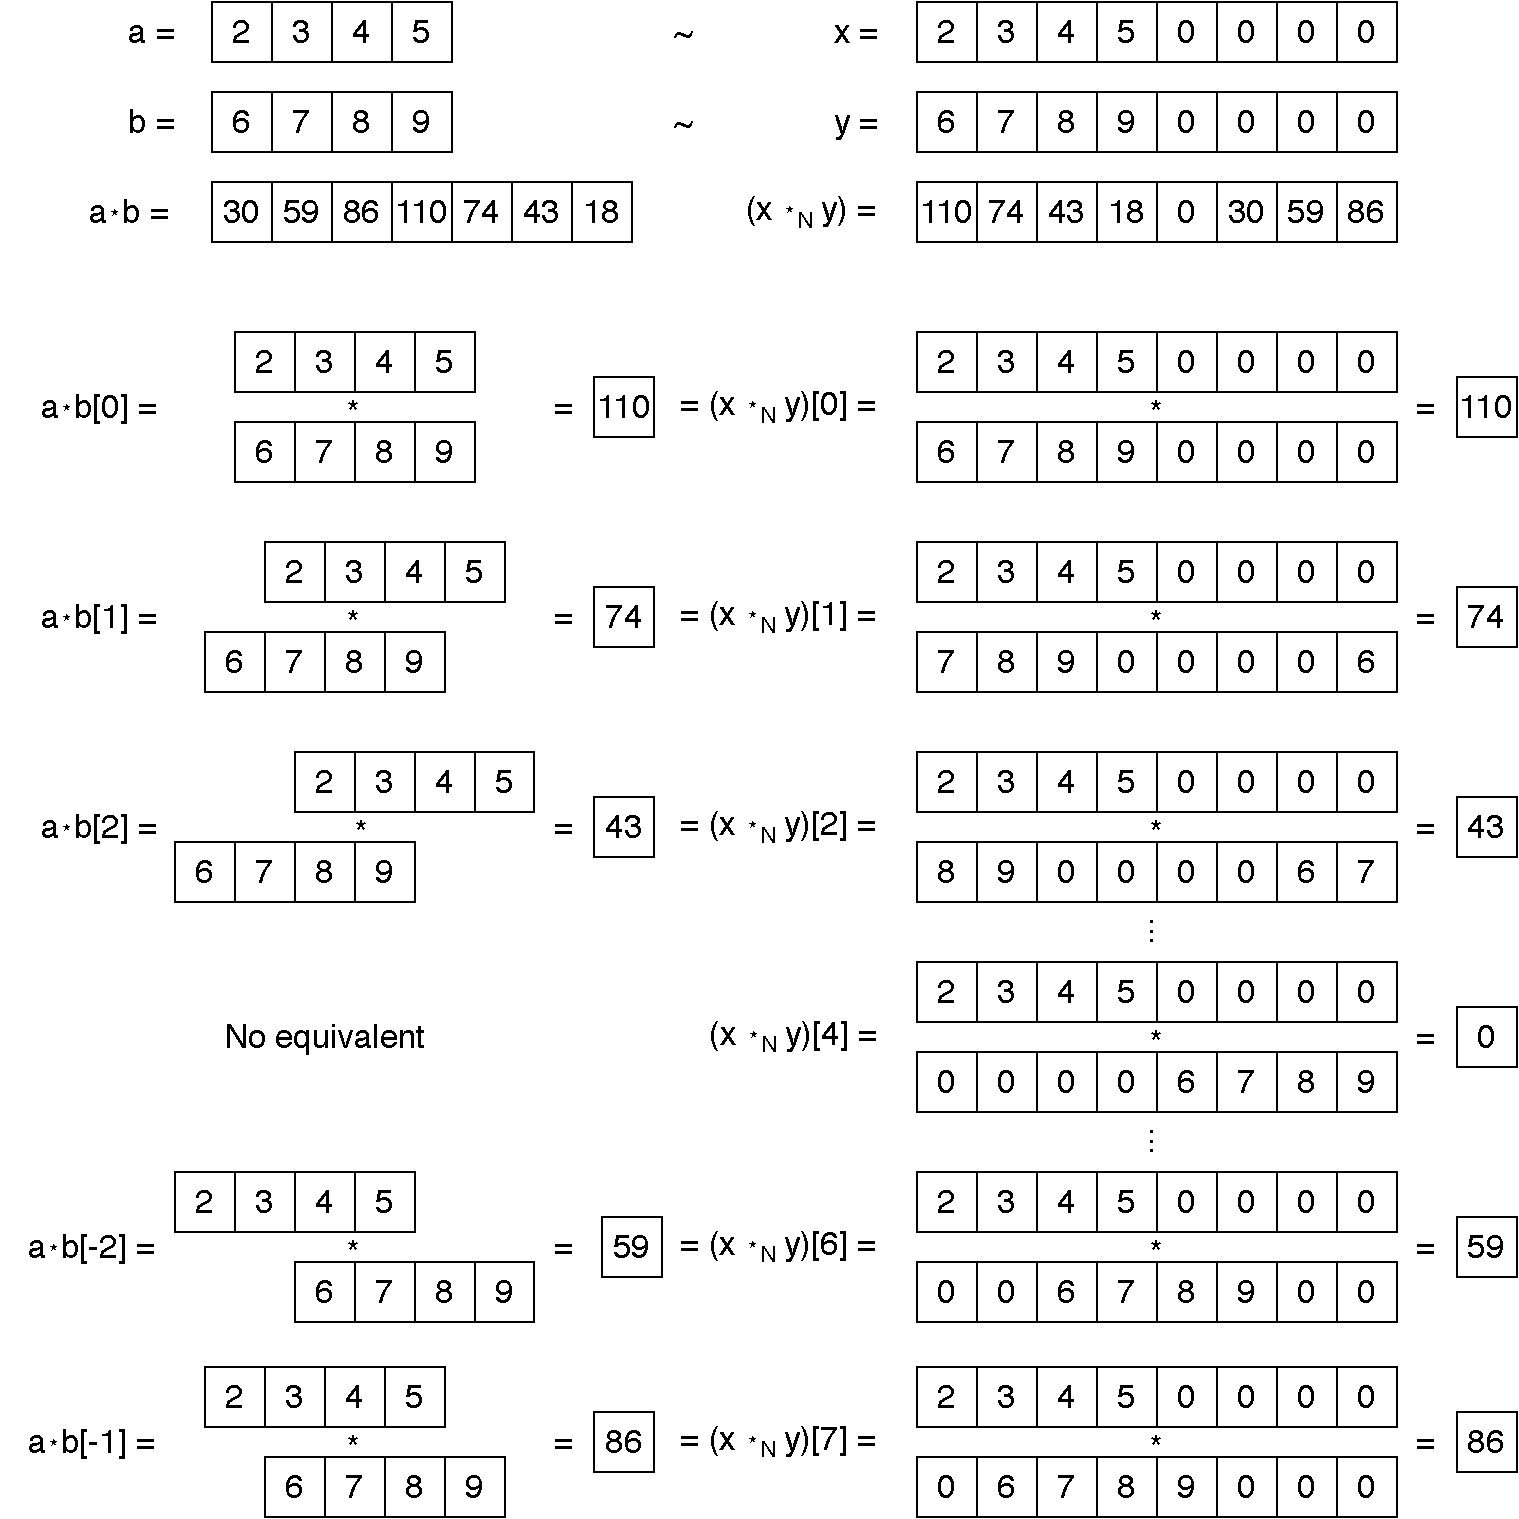
\includegraphics[width=\textwidth]{img/circ-cross-example}
	\caption{Illustration of the relationship between circular and non--circular cross--correlation. The left side shows a cross--correlation of two series $a$ and $b$. The right side shows the circular cross--correlation of $x$ and $y$, which are zero--padded versions of the series $a$ and $b$. Corresponding values of both correlations are shown side by side.}
	\label{circ-cross-example}
\end{figure}

To compute non--circular cross--correlation using this method, we use the following trick: for series $\{x_n\}$ and $\{y_n\}$ of length $N$, we expand both of them with $N$ zeros and then do circular cross--correlation. The result of such operation is the desired cross--correlation, only circularly shifted by N elements. The reason why it works is illustrated in \Cref{circ-cross-example}. When doing regular cross--correlation (in the left side of the figure), we slide one of the series along the other and for every shift, we multiply the corresponding numbers. If a number does not have any counterpart in the other series with respect to the current shift, it is discarded. For circular cross--correlation, we again slide one of the series, but this time we do it circularly using the modulo operator. We use the zeros that we expanded the original series with to rule out the values that should not be multiplied for the current shift.

The circular cross--correlation of zero--padded series results in a series $\{c_n\} = \mathbf{x} \star_N \mathbf{y}$ of $2N$ numbers. The numbers in the series have the following interpretation: $c_0, \cdots, c_{N-1}$ are the values of non--circular cross--correlation with shifts $0, 1, \cdots, N$ and $c_{N+1}, c_{N+2}, \cdots, c_{2N-1}$ represent the shifts $(-N+1), (-N+2), \cdots, -2, -1$. $c_{N}$ is always zero and does not have any interpretation.

\subsubsection{Two--dimensional discrete Fourier transform}
\label{two-dim-ft}
In order to use the described method in our implementation, we need to expand it to work on two--dimensional inputs.

Let $N, M \in \mathbb{N}$, $\mathbf{x} \in \mathbb{C}^{N\times M}$. Then $\mathbf{X} \in \mathbb{C}^{N\times M}$ is the Fourier transform of x, if the following holds for each item of the matrix $\mathbb{X}$:
\[
X_{k,l} = \sum_{n=0}^{N-1} \sum_{m=0}^{M-1} x_{n,m} \cdot e^{-i2\pi(\frac{kn}{N} + \frac{lm}{M})}.
\]

Next, the circular cross--correlation theorem can be rewritten for two dimensions as well. Let $N, M \in \mathbb{N}$, $\mathbf{x} \in \mathbb{C}^{N\times M}$, $\mathbf{y} \in \mathbb{C}^{N\times M}$ let $\mathbf{X} = \mathcal{F}(\mathbf{x})$ and $\mathbf{Y} = \mathcal{F}(\mathbf{y})$ be their Fourier transforms. Then, we can compute the two--dimensional circular cross--correlation like so: 
\[
\mathcal{F}^{-1}\{\mathbf{X}^\star \cdot \mathbf{Y}\}_{n,m} = \sum_{k=0}^{N-1} \sum_{l=0}^{M-1} x^\star_{k,l} y_{(n+k)\bmod N, (m+l)\bmod M},
\]
where $\cdot^\star$ denotes the complex conjugate and $\cdot$ denotes element by element multiplication.

The trick with zero--padding the inputs applies to the two--dimensional case as well. So when we want to compute the cross--correlation of two images $x$ and $y$ (represented by matrices in the theorem) with resolution $W \times H$, we do the following steps:
\begin{enumerate}
	\item Zero--pad the images --- we enlarge the image to the size $2W \times 2H$ by adding zeros.
	\item Compute the Fourier transforms of the images, which gives us two matrices $X = \mathcal{F}(x)$ and $Y =\mathcal{F}(y)$ of complex numbers with sizes $2W \times 2H$.
	\item Compute the complex conjugate of the matrix $X$.
	\item Multiply $X^\star$ with $Y$ element by element. The operation is also called \emph{Hadamard product}.
	\item Do the inverse discrete Fourier transform on the product.
\end{enumerate}
The result is a matrix $R$ of real numbers with the size $2W \times 2H$. It contains the cross--correlation of the input images, but it is circularly shifted. Similar to the one--dimensional case, where the item $N$ of the series was always zero, now the column $R_{*,N}$ and row $R_{N,*}$ are both zero. They separate the matrix into 4 quadrants that are circularly shifted by $N$ compared to the cross--correlation. Thus, the last step needed to get the resulting cross--correlation is to shift the matrix back by $N$, which is the same as swapping the quadrants diagonally.

\subsection{Zero--normalized cross--correlation}

Cross--correlation as we defined it (see \cref{cross-corr-def}) has a major flaw for image processing: it is heavily affected by the brightness of the images. Consider an image, that has some subregions brighter than others. Then, by definition of cross--correlation, that subregions add more to the result, regardless of the second image. \Cref{normalized-initial} shows an example of an image that is much brighter in the top part than in the bottom. \Cref{normalized-simple-cross} shows the result of cross--correlation with the search pattern in \cref{normalized-pattern}. It is clear that the highest values are located where the original image is brightest instead of locating the search pattern.

\begin{figure}
	\centering
	\begin{subfigure}{.5\textwidth}
		\centering
		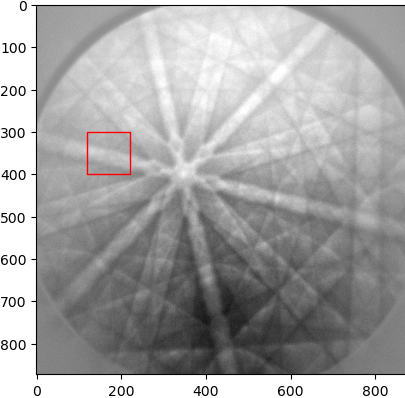
\includegraphics[width=\linewidth]{img/normalized_initial}
		\caption{An electron backscatter pattern}
		\label{normalized-initial}
	\end{subfigure}
	\begin{subfigure}{.4\textwidth}
		\centering
		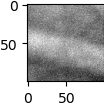
\includegraphics[width=0.4\linewidth]{img/normalized_pattern}
		\caption{Search pattern}
		\label{normalized-pattern}
	\end{subfigure}
	\begin{subfigure}{.49\textwidth}
		\centering
		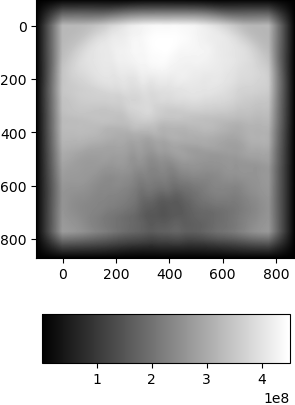
\includegraphics[width=\linewidth]{img/normalized_simple_corr}
		\caption{Simple cross--correlation}
		\label{normalized-simple-cross}
	\end{subfigure}
	\begin{subfigure}{.49\textwidth}
		\centering
		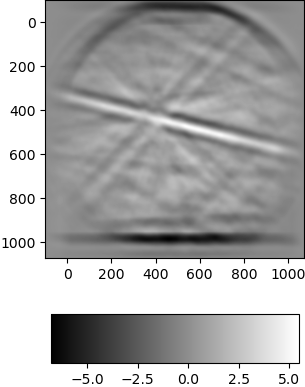
\includegraphics[width=\linewidth]{img/normalized_corr}
		\caption{Normalized cross--correlation}
		\label{normalized-cross}
	\end{subfigure}
	
	\caption{An image of backscatter pattern is correlated with its subregion, once using simple cross--correlation and once using the normalized cross--correlation.}
\end{figure}

That is why zero--normalized cross--correlation is used. It is based on subtracting respective means from each image. Normalized cross--correlation of two images $f$ and $g$ is defined as follows:
\[
\textsc{ZNCC}[i,j] = \sum_{x, y} \frac{1}{\sigma_f \sigma_g}(f[x,y] - \mu_f)(g[x+i,y+j] - \mu_g),
\]  
where $\mu_f$ and $\mu_g$ are the means of the images and $\sigma_f$, $\sigma_g$ are their standard deviations. For an image $f$ with size $W \times H$, they are defined as follows:
\begin{align*}
\mu_f &= \frac{1}{WH} \sum_{x,y}{}f[x,y], \\
\sigma_f &= \sqrt{\frac{1}{WH-1} \sum_{x,y}(f[x,y]-\mu_f)^2}.
\end{align*}

\Cref{normalized-cross} shows the zero--normalized cross--correlation of the figures \ref{normalized-initial} and \ref{normalized-pattern}. The area of the highest correlation is now clearly visible and corresponds to a Kukuchi line in the original image. Subtracting the mean of both images makes the algorithm less prone to brightness changes across the image.

The intuition behind this behavior is as follows. By the definition of simple cross--correlation, pixels with low brightness multiply and result in low correlation. After subtracting the means, low values in both images become negative. However, two negative numbers multiply into a positive value, so they increase the correlation. On contrary, very bright and very dark pixels multiply into a negative number so their difference causes that they lower the overall correlation value.

The zero--normalized cross--correlation is used in processing of the electron backscatter patterns to compare the reference deformed subregions. It can be computed in three steps:
\begin{enumerate}
	\item Find the means of the reference and deformed subregions
	\item Subtract the means from the pixels of both subregions
	\item Find the standard deviations of the reference and deformed subregions
	\item Divide the the pixels of both subregions by their respective standard deviations
	\item Compute the cross--correlation of the subregions
\end{enumerate}
First four steps normalize the subregions and then we perform the simple two--dimensional cross--correlation. The result is a two--dimensional matrix with size $(2W_s-1) \times (2H_s-1)$, if the subregions have size $W_s \times H_s$.


\section{Subpixel peak}
\label{subpixel-peak}
Next, we find the maximum of the cross--correlation. The location of the maximum $[x_m,y_m]$ in the matrix is the shift between the deformed and reference subregions. However, the precision of one pixel is not accurate enough in the context of the nanoworld the electron backscatter diffraction studies. That is why we use the cross--correlated data to estimate the maximum with subpixel accuracy.

We expect that if we could compute the cross--correlation with infinite resolution, so it would be continuous, the neighborhood of the maximum would look like a two--dimensional quadratic function with exactly one maximum. Since we only have limited resolution, we estimate~(fit) the continuous quadratic function from several discrete points of the cross--correlation --- the neighborhood of the maximum. The neighborhood is square--shaped and its size $F \times F$ is a parameter of the algorithm. Finally, we find the exact location of maximum of the estimated continuous quadratic function, which may be slightly shifted from the discrete maximum, depending on the values of the cross--correlation in the neighborhood.


So the processing of the cross--correlation is done in several steps:
\begin{enumerate}
	\item Find the position $[x_m,y_m]$ of the maximum (often denoted as \emph{arg max} operation) of the cross--correlation. It is a pair of whole numbers from the closed interval $(-W_s, W_s) \times (-H_s, H_s)$.
	\item Use the \emph{least squares method} to fit a quadratic function to the neighborhood of the maximum. The function is a continuous representation of the cross--correlation peak.
	\item Find the position of the maximum of the continuous function.
\end{enumerate}

In the following sections, we describe these steps in detail.

\subsection{Least squares}
The least squares method is used to approximate the solution of systems of equations which do not have an exact solution, since there are more equations than variables. Such systems are also called overdetermined systems. In the electron backscatter pattern analysis, the least squares method is used to approximate coefficients of a quadratic function from its several known points.

In the first place, let us formulate the problem that the least squares method addresses. Let $n,m \in \mathbb{N}, n > m; A \in \mathbb{R}^{n \times m}; x \in \mathbb{R}^m$ and $b \in \mathbb{R}^n$. Then $Ax = b$ is an overdetermined system of linear equations. It may have a solution, if $b$ is a linear combination of column vectors of $A$ ($b$ is in column space of $A$), but in general, that is not the case.

Instead of solving the system, we search for a vector $x'$ that has the least difference from the right hand side of the equation:
\[
x' = \min_x \norm{Ax - b},
\]
where $\norm{\cdot}$ denotes Euclidean norm. For a vector $x \in \mathbb{R}^n$, it is defined as:
\[
\norm{x} = \sqrt{\sum_{i=0}^{n} x_i^2}.
\]
So we minimize the sum of squared differences between the left and right sides of the equations in the system, hence the name least squares.

The least squares solution can be calculated using only matrix multiplication and inversion as follows \cite{anton2013elementary}:  
\[
x' = (A^TA)^{-1}A^Tb.
\]

This formula is not used in practice because of effectiveness and numerical stability (instead, it is better to solve the equation $A^TAx = A^Tb$). However, for the algorithm described in this thesis, the approach is sufficient, since the matrix $A$ is constant in our case (as we will explain in the end of \cref{estimation} for further explanation).

\subsection{Maximum neighborhood fitting}

We use the least squares method to estimate the coefficients of a two--dimensional quadratic function from the neighborhood of the cross--cor\-re\-la\-tion maximum. The neighborhood has size $F \times F$ and has the shape of a square, so for maximum at location $[x_m, y_m]$, the neighborhood points are at positions 
\[
\{x_m - \frac{F-1}{2}, \cdots, x_m, \cdots, x_m + \frac{F-1}{2}\} \times \{y_m - \frac{F-1}{2}, \cdots, y_m, \cdots, y_m + \frac{F-1}{2}\}.
\]
We only consider odd $F$, so the maximum is always in the middle.

The estimated two--dimensional quadratic function $f:\mathbb{R} \rightarrow \mathbb{R}$ can be written as as:
\[
f(x,y) = q_1 + q_2x + q_3y + q_4x^2 + q_5xy + q_6y^2,
\]
where $q_1 \dots q_6 \in \mathbb{R}$. To estimate such function is to find the 6 coefficients $q_1 \dots q_6$. From the known points of the neighborhood $N$ of size $F \times F$, it is possible to create the following system of equations:
\[
\forall [x,y] \in \{0,1,\dots , F-1\}^2 : q_1 + xq_2 + yq_3 + x^2q_4 + xyq_5 + y^2q_6 = N[x,y],
\]
where $q_1 \dots q_6$ are unknown variables.

So for each point with coordinates $[x,y]$ in the neighborhood, we create one equation with substituted $x$ and $y$. We have $F^2$ known points, from which we create $s^2$ equations. We have 6 unknown variables and $F$ has to be greater than one and odd, so we have more equations than unknowns. 

\subsubsection{Example of creating equation system}

For instance, let $F$ be 3 and $N$ be the neighborhood of the maximum:
\[
N =
\begin{bmatrix}
751 & 819 & 765 \\
825 & 934 & 810 \\
768 & 798 & 725
\end{bmatrix}.
\]


\iffalse
\[
\begin{bmatrix}
1 & 0 & 0 & 0 & 0 & 0\\
1 & 1 & 0 & 1 & 0 & 0\\
1 & 2 & 0 & 4 & 0 & 0\\
1 & 0 & 1 & 0 & 0 & 1\\
1 & 1 & 1 & 1 & 1 & 1\\
1 & 2 & 1 & 4 & 2 & 1\\
1 & 0 & 2 & 0 & 0 & 4\\
1 & 1 & 2 & 1 & 2 & 4\\
1 & 2 & 2 & 4 & 4 & 4
\end{bmatrix}
\cdot
\begin{bmatrix}
q_1 \\ q_2 \\ q_3 \\ q_4 \\ q_5 \\ q_6
\end{bmatrix}
=
\begin{bmatrix}
751 \\ 819 \\ 765 \\ 825 \\ 934 \\ 810 \\ 768 \\ 798 \\ 725
\end{bmatrix}.
\]
\fi

Then, the linear system looks like this:
\begin{align*}
x=0,y=0 \rightarrow q_1 + 0q_2 + 0q_3 + 0q_4 + 0q_5 + 0q_6 &= N[0,0] = 751 \\
x=1,y=0 \rightarrow q_1 + 1q_2 + 0q_3 + 1q_4 + 0q_5 + 0q_6 &= N[1,0] = 819 \\
x=2,y=0 \rightarrow q_1 + 2q_2 + 0q_3 + 4q_4 + 0q_5 + 0q_6 &= N[2,0] = 765 \\
x=0,y=1 \rightarrow q_1 + 0q_2 + 1q_3 + 0q_4 + 0q_5 + 1q_6 &= N[0,1] = 825 \\
x=1,y=1 \rightarrow q_1 + 1q_2 + 1q_3 + 1q_4 + 1q_5 + 1q_6 &= N[1,1] = 934 \\
x=2,y=1 \rightarrow q_1 + 2q_2 + 0q_3 + 4q_4 + 2q_5 + 1q_6 &= N[2,1] = 810 \\
x=0,y=2 \rightarrow q_1 + 0q_2 + 2q_3 + 0q_4 + 0q_5 + 4q_6 &= N[0,2] = 768 \\
x=1,y=2 \rightarrow q_1 + 1q_2 + 2q_3 + 1q_4 + 2q_5 + 4q_6 &= N[1,2] = 798 \\
x=2,y=2 \rightarrow q_1 + 2q_2 + 2q_3 + 4q_4 + 4q_5 + 4q_6 &= N[2,2] = 725 \\
\end{align*}

The left sides contains the equation of the two--dimensional quadratic function with substituted points from the set $\{0,1,2\}^2$ (for this example, we have chosen the zero point to be the top left corner). The right side contains all the corresponding values from neighborhood $N$.

\subsubsection{Estimation of function coefficients using least squares method}
\label{estimation}

Once we create the system of equations, we solve it using the least squares method. Recall its solution:
\[
x' = (A^TA)^{-1}A^Tb.
\]
Matrix $A$ in the solution corresponds to the left sides of the system of equations, $b$ is the vector with values of the neighborhood. We can observe that the left sides of the equations (matrix $A$) are constant for any neighborhood of size $F$. That also implies that the expression $(A^TA)^{-1}A^T$ in the least squares solution is constant for the values of the neighborhood and only depends on the parameter $F$.

That means we can precompute the constant part of the least squares formula for each $F$. That reduces the computation of least squares to only one matrix--vector multiplication. We do not expect that $F$ can have many different values. It has to be odd and the neighborhood is expected to be fairly small --- for this thesis we implemented only the options $F \in \{3, 5, 7, 9\}$.


\subsection{Maximum of fitted function}
\label{max-fitted}
The last step in the algorithm is to find the maximum of the quadratic function. We do that using standard methods of mathematical analysis: we find where are the partial derivations of the function equal to zero.

The partial derivations of the quadratic function are:
\begin{align*}
\frac{\partial f}{\partial x}(x,y) &= 2q_4x + q_5y + q_2,\\
\frac{\partial f}{\partial y}(x,y) &= q_5x + 2q_6y + q_3.
\end{align*}

If the function has an extreme, then it is located at the point where the partial derivations are both zero. That implies a linear system of equations with the following solution:
\begin{align*}
x_m &= \frac{2q_2q_6 - q_3q_5}{q_5^2 - 4q_4q_6}\\
y_m &= \frac{2q_3q_4 - q_2q_5}{q_5^2 - 4q_4q_6}
\end{align*}

The point $[x_m, y_m]$ is the maximum of the function fitted to the neighborhood of the cross--correlation maximum.

\subsubsection{Scaling the neighborhood by constant}

When we multiply the result of the cross--correlation by constant, the result of the algorithm does not change. The reason is as follows. In the first step of the algorithm, we find the position of maximum of the cross--correlation which is not affected by constant scaling. Next, since the neighborhood is scaled by constant, the quadratic function approximation will be scaled as well. Finally, we find the maximum position of the estimated continuous function, which is the same as if the function was not scaled.

It means that when computing the zero--normalized cross--correlation, we can omit two of its steps --- computation of standard deviation and division by the result, which simplifies the final algorithm.

\section{Summary}
\label{algo-summary}
Algorithm \ref{algo-whole} summarizes the algorithm described in this chapter. It is clear that all the patterns and even their subregions are processed separately so it is easy to parallelize it. At the same time, there may be thousands of the patterns and tens of subregions in each, so there is enough data to utilize the whole GPU. The most computationally expensive part is the cross--correlation. We explain the implementation details of the algorithm in the next chapter.

\begin{algorithm}
	\caption{EBSP deformation processing}
	\label{algo-whole}
	\KwIn{one reference electron backscatter pattern \newline
		$N$ deformed electron backscatter patterns \newline
		position of $M$ subregions from each pattern \newline
		size of a subregion \newline
		parameter $F$ --- size of neighborhood}
	\KwOut{deformation shifts for all $M$ subregions from all $N$ deformed patterns}
	\vspace{5px}
	
	refPat  $\leftarrow$ load reference pattern from disk\;
	\ForEach{deformed pattern}{
		defEBSP $\leftarrow$ load deformed pattern from disk\;
		\ForEach{\emph{regPos} in subregion positions}{
			refReg $\leftarrow$ extract subregion at regPos from refPat\;
			defReg $\leftarrow$ extract subregion at regPos from defPat\;
			\BlankLine
			refMean, defMean $\leftarrow$ means of both subregions\;
			\BlankLine
			subtract refMean from pixels of refReg\;
			subtract defMean from pixels of defReg\;
			\BlankLine
			crossResult $\leftarrow$ cross--correlate(refReg,defReg)\;
			\BlankLine
			maxX, maxY $\leftarrow$ subpixelPeak(crossResult)\;
			output [maxX, maxY]\;
		}
	}
	
	\SetKwProg{Fn}{Function}{}{end}
	\SetKwFunction{FSubpixelPeak}{subpixelPeak}    
	\Fn{\FSubpixelPeak{crossResult}}{
		[maxX, maxY] $\leftarrow$ argmax(crossResult)\;
		neighbors $\leftarrow$ extract neighborhood of [maxX, maxY]\;
		
		coefs $\leftarrow$ fitQuadraticFunction($F$, neighbors)\;
		\KwRet arg max of the quadratic function with coefficients coefs \;
	}
\end{algorithm}

